\begin{center}
	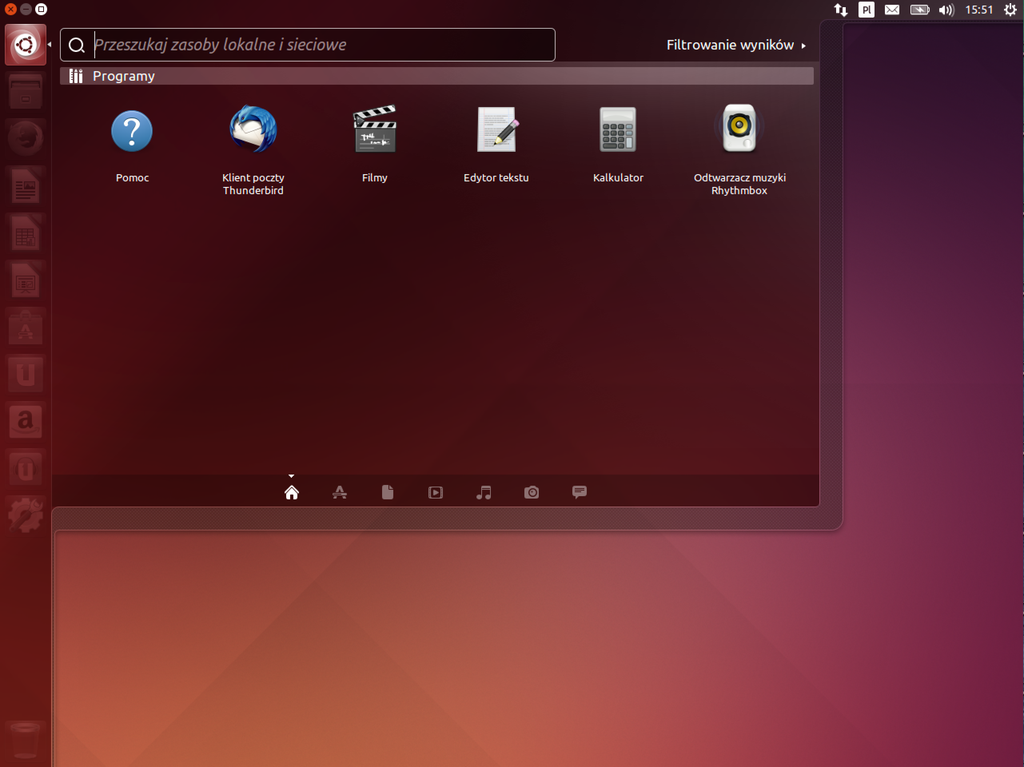
\includegraphics[width=\linewidth]{images/unity_pulpit_dash.png}
\end{center}

Dash jest potężnym narzędziem Unity, pozwalającym na szybkie wyszukiwanie i łatwy dostęp do programów, plików oraz dodatkowych informacji przechowywanych nie tylko w naszym komputerze (zainstalowane programy, ostatnio używane dokumenty, zakładki, ostatnio odwiedzone strony i inne), ale również dostępnych w sieci (Twitter, Facebook, Google Docs, Youtube, Wikipedia, Amazon i inne). Wyniki wyszukiwania w zewnętrznych serwisach dopasowane są do wyszukiwanej frazy i zwracane w oknie Dasha. Jeżeli niepokoi cię, że szukana fraza przesyłana jest do internetu, to możesz tę funkcję wyłączyć w Ustawieniach systemowych, w oknie \textcolor{ubuntu_orange}{Prywatność i bezpieczeństwo}.

Dash można porównać do Menu Start z systemu Microsoft Windows XP/Vista/7 lub do ekranu startowego w Windows 8. Odpowiednikiem Dasha w systemie Mac OS X jest Launchpad.

\begin{wrapfigure}{l}{0.1\textwidth}
	\vspace{-10pt}
	
\includegraphics[width=\linewidth]{images/ikony_dash.png}
\end{wrapfigure}

Ikona Dasha umieszczona jest na pierwszej pozycji na pasku Launchera --- jest ona dość charakterystyczna i zawiera logo Ubuntu. Po naciśnięciu ikony Dasha pojawi się jego przezroczyste okno, które w środkowej części wyświetla dwie grupy: ostatnio uruchomionych programów, ostatnio przeglądanych oraz pobranych plików i katalogów, a także wyszukiwanych informacji. W górnej części Dasha znajduje się pasek wyszukiwania, który pozwala przeszukiwać nie tylko zasoby komputera, ale również wyszukiwać i przeglądać informacje z popularnych serwisów w sieci. 

\begin{wrapfigure}{l}{0.2\textwidth}
                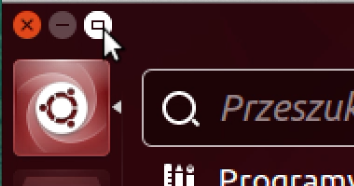
\includegraphics[width=\linewidth]{images/unity_dash_max.png}
\end{wrapfigure}

Dash po uruchomieniu zajmuje pewien obszar ekranu. Jego okno można powiększyć na cały ekran --- służy do tego przycisk maksymalizacji w lewym górnym rogu, widoczny, gdy Dash jest aktywny.\\
Wyszukiwanie w pasku jest dynamiczne i rezultaty zmieniają się podczas wpisywania tekstu, a wyniki można filtrować. Służy do tego nie tylko przycisk filtrowania wyników, ale również domyślnie włączone soczewki (Lenses).

\subsubsection{Soczewki (Lenses)}
\begin{center}
	
\includegraphics[width=\linewidth]{images/unity_dash_lenses.png}
\end{center}

Domyślnie w systemie dostępnych jest siedem soczewek, których ikony widoczne są na dole okna Dasha. Aktualnie wybrana soczewka jest jaśniejsza od pozostałych, a nad nią widać niewielki trójkącik. Soczewki służą do ograniczania wyników wyszukiwania do konkretnych kategorii.
\begin{description}
\item[
\includegraphics{images/unity_dash_lens_home.png}] \textcolor{ubuntu_orange}{Soczewka domowa} --- zawiera wszystkie wyniki wyszukiwania. 
\item[
\includegraphics{images/unity_dash_lens_programy.png}]\textcolor{ubuntu_orange}{Soczewka programów} --- zawiera wyniki wyszukiwania programów.
\item[
\includegraphics{images/unity_dash_lens_pliki.png}] \textcolor{ubuntu_orange}{Soczewka plików} --- zawiera wyniki wyszukiwania plików i katalogów.
\item[
\includegraphics{images/unity_dash_lens_video.png}] \textcolor{ubuntu_orange}{Soczewka filmów} --- zawiera wyniki wyszukiwania filmów.
\item[
\includegraphics{images/unity_dash_lens_audio.png}] \textcolor{ubuntu_orange}{Soczewka muzyki} --- zawiera wyniki wyszukiwania muzyki.
\item[
\includegraphics{images/unity_dash_lens_photo.png}] \textcolor{ubuntu_orange}{Soczewka zdjęć} --- zawiera wyniki wyszukiwania fotografii.
\item[
\includegraphics{images/unity_dash_lens_social.png}] \textbf{Soczewka społecznościowa} --- zawiera wyniki wyszukiwania w serwisach społecznościowych, do których jesteś zalogowany.
\end{description}

Soczewka domowa ma wiele zastosowań --- oprócz wcześniej wspomnianych możliwości, możemy ją wykorzystać do wyszukania informacji na przykład w Wikipedii, Google, lub możemy wyszukać informacje na temat pogody w naszym regionie.
\clearpage
\begin{center}
	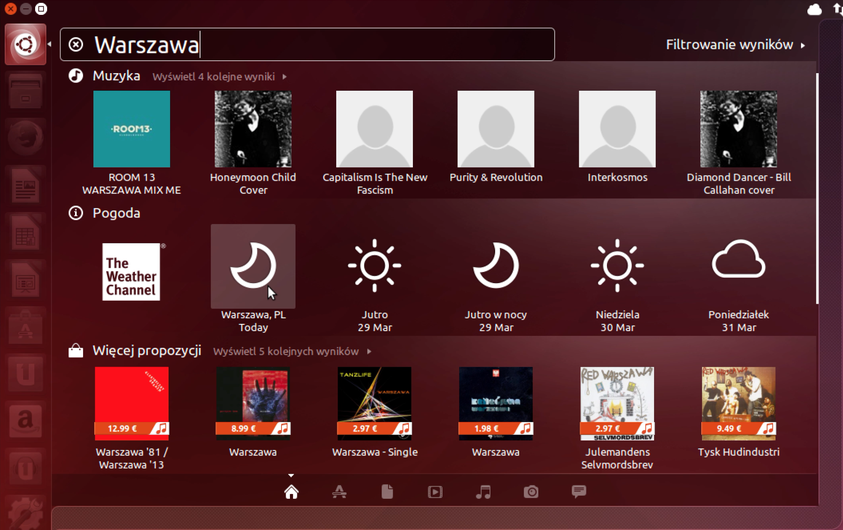
\includegraphics[width=\linewidth]{images/unity_dash_wyszukiwanie.png}
\end{center}

Aby uzyskać więcej informacji, nie trzeba od razu otwierać wyniku. Naciśnięcie prawym przyciskiem myszy któregoś z wyników wyszukiwania spowoduje wyświetlenie większej ilości informacji.

\begin{center}
	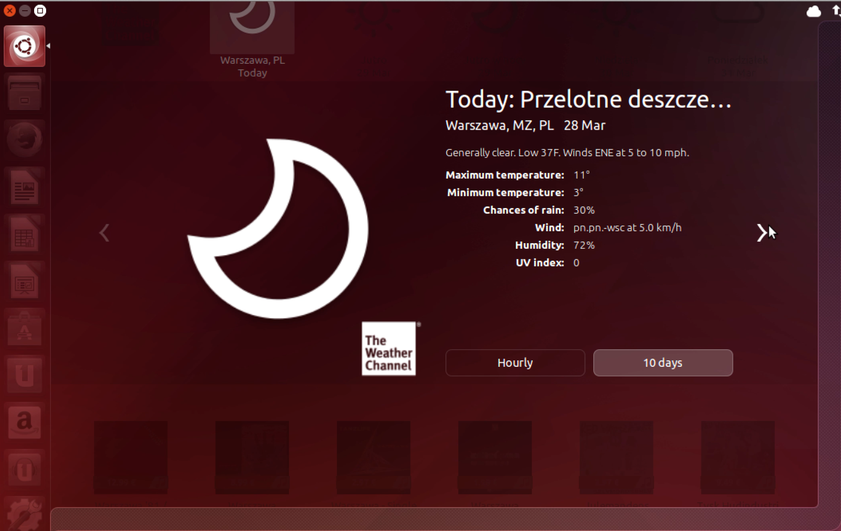
\includegraphics[width=\linewidth]{images/unity_dash_wyszukiwanie2.png}
\end{center}

Wyniki wyszukiwania można zawęzić do konkretnych źródeł, wykorzystując do tego przycisk filtrowania wyników. Podobnie jest w przypadku wyszukiwania informacji z wykorzystaniem pozostałych soczewek.

\begin{center}
	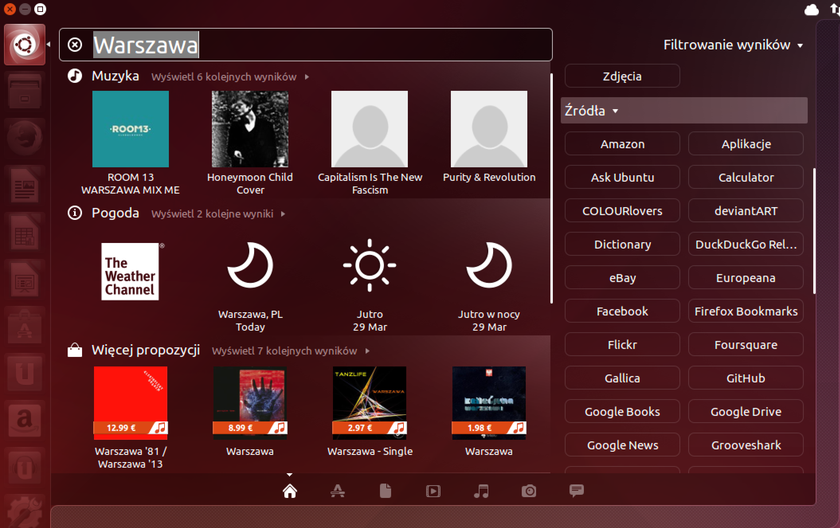
\includegraphics[width=\linewidth]{images/unity_dash_wyszukiwanie3.png}
\end{center}

W Ubuntu nie jesteśmy ograniczeni do domyślnego zestawu soczewek. Wiele serwisów internetowych udostępnia swoje własne soczewki, które można w łatwy sposób doinstalować i korzystać z nich w ten sam sposób, jak z domyślnych.
%TODO opisać instalację soczewki.
